% Author: Emmanuel D. Solis
\documentclass{article}

% Set font encoding for PDFLaTeX, XeLaTeX, or LuaTeX
\usepackage{ifxetex,ifluatex}
\if\ifxetex T\else\ifluatex T\else F\fi\fi T%
  \usepackage{fontspec}
\else
  \usepackage[T1]{fontenc}
  \usepackage[utf8]{inputenc}
  \usepackage{lmodern}
\fi

%--------- Bibliografias --------
\usepackage{apacite} %Trabajar bibliografias APA
\usepackage{natbib} %Agregar Bibliografias

%------------ Estilos -----------
\usepackage{afterpage} %Agregar paginas en blanco
\usepackage{bookmark} %Para bookmark del indice
\usepackage[shortlabels]{enumitem} %Para enumerar con letras
\usepackage{float} %Tablas y posicionamiento de figuras.
\usepackage{fullpage} %Trabajar con menos margenes de pagina
\usepackage{graphicx} %Agregar imagenes
\usepackage{hyperref} %Uso de vinculos
\usepackage{pdfpages} %Incluir pdf externos
\usepackage{xcolor}  %Usar colores

%---------- Herramientas ----------
\usepackage{amsfonts} %Formulas matematicas
\usepackage{amsmath} %Alinear ecuaciones y similar.
\usepackage{listings} %Comandos de Terminal UNIX.
\usepackage{minted} %Incluir codigo de programacion.
\usemintedstyle{one-dark} %Estilo de codigo de programacion.
%\usepackage{sagetex} %Hacer calculos
\usepackage{venndiagram} %Agregar diagramas de Venn

%----------- Idiomas ---------------
\usepackage[spanish]{babel} %Configurar el idioma

\begin{document}

\begin{titlepage}
\centering
{
\includegraphics[width=0.2\textwidth]{logoUCR.png}\par}
\vspace{1cm}
{\bfseries\LARGE Universidad de Costa Rica \par}
\vspace{1cm}
{\scshape\Large Facultad de Ingenier\'ia \par}
{\scshape\Large Escuela de Ciencias de la Computaci\'on e Inform\'atica \par}
\vspace{1cm}
{\scshape\Large CI0128 – Proyecto Integrador: Ingeniería de Software y Bases de Datos \par}
{\scshape\Large Profesoras: Rebeca Obando y Alexandra Martínez \par}
\vspace{1cm}
{\scshape\Huge Reporte: Sprint 2 \par}
\vspace{1cm}
{\Large Nombre del Equipo: Ta' Bueno \par}
\vspace{0.5cm}
{\Large Miembros: \par}
{\Large Emmanuel D. Sol\'is - B97670 (Scrum Master)\par}
{\Large \textit{\color{blue}emmanuel.solispomares@ucr.ac.cr} \par}
{\Large Gabriel Zúñiga - B98755\par}
{\Large \textit{\color{blue}gabriel.zunigaorozco@ucr.ac.cr} \par}
{\Large Jan Murillo - B95447\par}
{\Large \textit{\color{blue}jan.murillo@ucr.ac.cr} \par}
{\Large Kevin Arguedas - B80626\par}
{\Large \textit{\color{blue}kevin.arguedasmuriel@ucr.ac.cr} \par}
{\Large Luis D. Chinchilla - B82227\par}
{\Large \textit{\color{blue}luis.chinchillaotarola@ucr.ac.cr} \par}
\end{titlepage}

%\newpage
% \tableofcontents

%\newpage
%\includepdf[pages={-}]{Enunciado.pdf}

\section{Código Fuente del Sistema}
Se encuentra tanto adjunto en esta carpeta compromida como en el enlace del GitHub
previamente compartido.

\section{Code Review}
A ser entregado el lunes 27 de junio por medio del correo institucional según
indicación de la profesora; véase Figura \ref{fig:message}.

\begin{figure}[h]
 \centering
 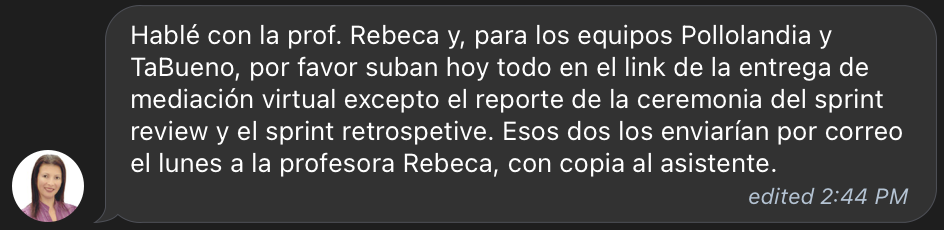
\includegraphics[width=0.95\textwidth]{message.png}
 \caption{Mensaje de la profesora Alexandra sobre indicaciones especiales de entrega de algunos rubros.}
 \label{fig:message}
\end{figure}

\section{Unit Testing}
Proyecto de pruebas se encuentra en la carpeta \textit{/Planilla/planilla\-backend\_testing}.

\section{Sprint Backlog}
Se encuentra en el siguiente enlace de la profesora Rebeca Obando: \url{https://ingesoftg001.atlassian.net/jira/software/projects/TB/boards/5/backlog}.

\section{Entregable de las ceremonias}
A ser entregado el lunes 27 de junio por medio del correo institucional según
indicación de la profesora; véase Figura \ref{fig:message}.

\section{Mock Ups}
Se encuentran en el archivo \textit{sprint2/mock\_ups.pdf}.

\section{Diagrama UML}
Se encuentran en el archivo \textit{sprint2/payment\_diagram.pdf}; véase Figura \ref{fig:message2}.

\begin{figure}[h]
  \centering
  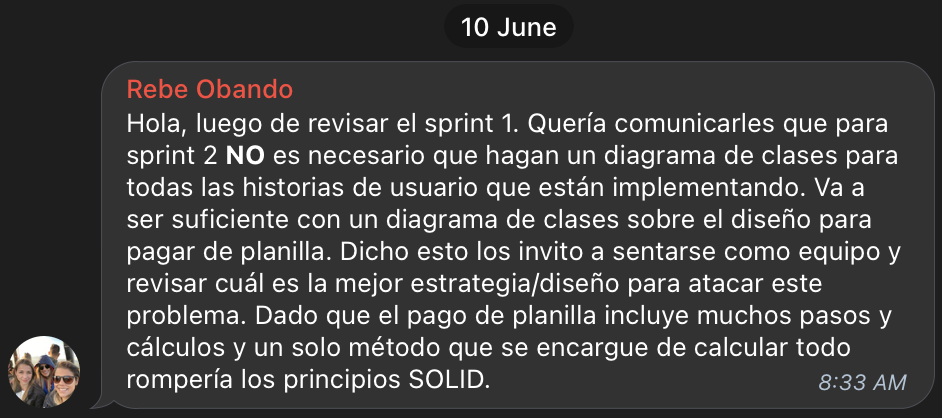
\includegraphics[width=0.85\textwidth]{message2.png}
  \caption{Mensaje de la profesora Rebeca sobre indicaciones especiales de entrega del diagrama de clases UML.}
  \label{fig:message2}
 \end{figure}

 \section{Implementación de la Base de Datos}
Nuestra base de datos \textit{Ta Bueno} se encuentra implementada con las tablas que teníamos
en los diagramas de Modelo Entidad\-Relación y Lógico que fueron previamente presentados y aprobados por la profesora 
Alexandra, los diagramas se encuentran adjuntos en el archivo \textit{sprint2/database\_diagrams.pdf}.

También se adjuntan los scripts que fueron usados para la creación de tablas, funciones, procedimientos 
y demás de la base de datos; estos se encuentran dentro de la carpeta \textit{sprint2/database\_scripts/}.

\section{Presentación durante Sprint Review}
Se realizará la exposición el día 27 de Julio del 2022 debido a problemas técnicos con la 
base de datos fuera de nuestro alcance.

\section{Autoevaluación y Coevaluación}
Cada miembro del equipo se encarga individualmente de enviar su documento de auto y coevaluación.

%\begin{figure}[h]
%  \centering
%  \includegraphics[width=0.65\textwidth]{SystemCalls.png}
%  \caption{Funcionamiento interno de una interrupción al Sistema Operativo \cite[]{whatSysCalls}.}
%  \label{fig:HowWorksSysCalls}
%\end{figure}

%---------------------- Document Ending ----------------------------------
\newpage
\bibliographystyle{apacite}
\bibliography{bibliography.bib}
\end{document}